In this section we present empirical evaluation that analyzes the impact of \textsc{Dms} on manual effort needed for test case labeling, and compares our approach with multiple previous test case prioritization methods.

In particular, our seek for answers to the following two research questions:

%\subsection{Research Questions}\label{sec.exp.rqs}

\begin{enumerate}[RQ1]
\item What is the effectiveness of \textsc{Dms} on single-fault programs?
\item What is the effectiveness of \textsc{Dms} on multi-fault programs?
\end{enumerate}

Section~\ref{sec.rq1} shows our experimental results that answer the first research question. Section~\ref{sec.rq2} presents answers to the second research question. Section~\ref{sec.exp.threats} describe the discussion and some threats to validity.


\subsection{RQ1: Single-Fault Programs}\label{sec.rq1}
Section~\ref{sec.exp.setup} gives details about our experimental setup for single-fault programs.
In Section~\ref{sec.exp.subject}, we introduce the subject programs used in our study. Sections~\ref{sec.exp.resultsA}~\&~\ref{sec.exp.resultsB} show the results.

\subsubsection{Experimental Setups and Measures}\label{sec.exp.setup}

In our experiment, every test case prioritization technique starts from
an arbitrary labeled failed trace because developers start debugging only when
test cases fail.

In this paper, we use \textsc{Raptor} as the bootstrapping technique ($\mathcal{P}$ in Figure \ref{algo:DMS}). During the bootstrapping process, $w$ is set to 10 to facilitate trend analysis. 

Following \cite{JiangCT11}, for each faulty version, we repeat each prioritization technique 20 times to obtain its average cost. For each time, a randomly chosen failed trace is used as the starting point to alleviate the sensitivity of the technique to the choice of starting traces. On the other hand, to fairly compare our approach with other prioritization methods, the {\em same randomly} chosen failed traces are used as the starting traces for all methods.

The effectiveness of test case prioritization methods would be manifested as the effectiveness of the subsequent fault localization results. 
So one way to compare the effectiveness of different prioritization methods based on the different diagnostic costs of the subsequently applied fault localization technique when the same number of test cases are selected by the different prioritization methods. In the literature, many fault localization studies use the percentage of program elements that need to be inspected according to the ranked list of fault localization results to locate all faults as one kind of diagnostic costs,
which is defined as follows:

\begin{equation}\label{equation.avgcost}
	cost = \dfrac{\left|  \left\{ j \left| \right. f_{T_{\mathcal{S}}}(d_j) \geq f_{T_{\mathcal{S}}}(d_*) \right\}  \right|}{\left|  \mathcal{D} \right|}
\end{equation}
where $\mathcal{D}$ consists of all program elements appearing in the program and $d_*$ represents the fault(s) (i.e., the root cause(s) of failures) of a program.
We calculate the average cost as the percentage of elements that developers have
to examine until locating the root causes ($d_*$) of failures. The lower the cost is, the better a fault localization technique is. 
Since multiple
program elements can be assigned with the same suspicious score, the numerator
is considered as the number of program elements $d_j$ that have bigger or the
same suspicious score to $d_*$. 

We can also define the {\em accuracy} of a fault localization technique as the reverse of the cost, which is the higher the better:

\begin{equation}\label{equation.accuracy}
	accuracy = 1 - cost
\end{equation}
In the following parts of the paper, we thus use {\em cost} and {\em accuracy} interchangeably when the context is clear.\footnote{There are a number of other ways to define diagnostic costs and accuracies, such as .... We chose the one in Equation \ref{equation.avgcost} and \ref{equation.accuracy} as they are commonly used and easy to understand.}

Another way to measure the effectiveness of test case prioritization methods is to see how many test cases can be reduced by each method.
A major goal of our paper is to minimize the number of test cases that need manual labelling but can maintain fault localization accuracies. So, in the following evaluation results, we also show the numbers of reduced test cases {\em with respect to a targeted fault localization cost (or accuracy)}.

If labeling all test cases and performing fault localization on all program spectra results in an average diagnostic cost $c$, we call it the {\em base line cost}. If a test prioritization technique or fault localization technique leads to a diagnostic cost $c'$, then we say the technique achieves {\em $x$\% of base line effectiveness}, where $x$ is defined as follows:

\begin{equation}\label{equation.baselinecost}
	x = \frac{c'}{c} \times 100
\end{equation}

To be fair, the number of reduced test cases by each prioritization technique should be measured when the technique achieves 100\% of base line effectiveness. However, in reality, it is hardly possible to directly control the cost to be exactly 100\% of base line. So, we allow 1\% deviation; i.e., in the following evaluation results, we measure the numbers of reduced test cases {\em when at most 101\% of base line effectiveness is achieved}.


\subsubsection{Subject Programs}\label{sec.exp.subject}

We use five real {\em C} programs and seven Siemens test programs from the
{\em Software-artifact Infrastructure Repository}~(SIR)~\citep{doESE05}. We refer to the five real programs (\texttt{sed}, \texttt{flex}, \texttt{grep}, \texttt{gzip}, and \texttt{space}) as \textsc{Unix} programs. Table \ref{dataset} shows the descriptive statistics of each subject,
including the number of faults, available test cases and code sizes. Following many previous studies \citep[e.g.][]{JHS02,Abreu:2009.jss}, we exclude faults not directly observable by the {\tt gcov} profiling
tool\footnote{http://gcc.gnu.org/onlinedocs/gcc/Gcov.html} (e.g., some faults lead to a crash before \texttt{gcov} dumps profiling information and some faults do not cause any test case to fail), and in total we study 254 faults.

\begin{table}[!htbp]
	%\vspace{-8pt}
	\centering
	\caption{Subject Programs}
	\renewcommand{\arraystretch}{1.5}
	\small
    \begin{tabular}{|l|c|c|c|c|} \hline
        Program & Description & LOC  & Tests & Faults\\ \hline\hline
		tcas & Aircraft Control & 173 & 1609 & 41\\ \hline
        schedule2 & Priority Scheduler & 374  & 2710  & 8\\ \hline
        schedule & Priority Scheduler & 412 & 2651  & 8\\ \hline
        replace & Pattern Matcher & 564 & 5543  & 31\\ \hline
		tot\_info & Info Measure & 565 & 1052  & 22\\ \hline
        print\_tokens2 & Lexical Analyzer & 570  & 4055  & 10\\ \hline
        print\_tokens & Lexical Analyzer & 726 & 4070  & 7\\ \hline
        space & ADL Compiler & 9564 & 1343 & 30\\ \hline
        flex & Lexical Parser & 10124 & 567  & 43\\ \hline
        sed & Text Processor & 9289  & 371  & 22\\ \hline
        grep & Text Processor & 9089 & 809  & 17\\ \hline
        gzip & Data Compressor & 5159 & 217  & 15\\ \hline
	\end{tabular}
	\label{dataset}
\end{table}

\subsubsection{Experimental Results: Reducing Number of Test Cases}\label{sec.exp.resultsA}
%In this subsection, we conduct several controlled experiments to show the effectiveness of \textsc{Dms}.

%\vspace{-4pt}
%\subsubsubsection{Effectiveness on Reducing The Number of Test Cases Needed for a Target Cost}

Here, we investigate the effectiveness of \textsc{Dms} in reducing the number of test cases needed for a targeted diagnostic cost. We compare \textsc{Dms} with previous test case prioritization techniques in terms of labeling effort when to achieve 101\% of base line effectiveness as stated in Section \ref{sec.exp.setup}.
%\lx{moved to setup section to explain our metrics.}
%given an expected fault localization accuracy.
%Since the major objective of our solution is to save labelling effort at the same time retain acceptable fault localization accuracy.
%If labeling all test cases and performing fault localization on all program spectra results in an average diagnostic cost $c$, we call it the base line cost. Then we define $x$\% base line effectiveness ($c_x$) as follows:

%\begin{equation}\label{equation.accu_cost}
%	c_{x} = \frac{x}{100} \times c
%\end{equation}

Since Dms would output a ranked list of suspicious program elements, we compute the diagnostic cost $c_n$ for {\sc Dms} when we just inspect top $n$ ($n \in \{1,2,\cdot \cdot \cdot, |D|\}$) suspicious elements. We record the {\em maximum} $n$ that $c_n$ is still within 101\% of base line cost as the amount of labeling effort. Also, we limit the maximum number of test cases allowed to select (i.e., $k$ in Algorithm \ref{algo:DMS}) to 500 in this specific evaluation.

Table \ref{tab:label_effort} shows how many labels are needed on average to achieve 101\% of base line effectiveness
% (i.e., within 1\% accuracy lost) 
for each approach.
E.g., \textsc{Raptor} requires 48 labels on average for each faulty version from the 5 \textsc{Unix} programs while \textsc{Dms} only needs 16.
Overall, \textsc{Dms} requires the minimal amount of labeling effort by achieving 67.7\% labeling reduction on \textsc{Unix}
programs and 10\% reduction on Siemens programs in comparison with the existing best approach (\textsc{Raptor}).

\begin{table}[tbp]
	%\vspace{-8pt}
	\centering
	\caption{Labeling Effort on Subject Programs}
{
	\scriptsize
		\renewcommand{\arraystretch}{1.5}
%		\hspace{-10pt}
        \begin{tabular}{|m{32pt}|m{13pt}|c|c|m{21pt}|m{21pt}|m{21pt}|m{17pt}|}
		   \hline
		     Subject &             &                &                  & \textsc{Stmt-} & \textsc{Stmt-} & \textsc{Fep-}  & \textsc{Art-} \\
		   Programs & \textsc{Dms} & \textsc{Raptor}  & \textsc{Sequoia} & \textsc{Addtl} & \textsc{Total} & \textsc{Addtl} & \textsc{Min} \\
		   \hline\hline
		   Siemens &   {\bf 18} &         20 &       500\tiny{+} &       500\tiny{+} &       500\tiny{+} &         97 &        150 \\
		   \hline
			\textsc{Unix} &   {\bf 16} &         48 &    176 &        150 &       500\tiny{+} &         98 &         56 \\
		   \hline
		\end{tabular}
}
	\label{tab:label_effort}
\end{table}


%\vspace{-6pt}
\subsubsection{Experimental Results: Reducing Cost}\label{sec.exp.resultsB}
%\subsubsubsection{Effectiveness on Reducing Cost for a Given Number of Labeled Test Cases}

Here, we investigate the effectiveness of \textsc{Dms} in reducing cost given a targeted number of labeled test cases. We select 30 test cases (i.e., set $k=30$ in Algorithm \ref{algo:DMS}), which we believe are not too many to manually label. We also find that in our experiments the average debugging cost of using \textsc{Dms} will not reduce noticeably even if more labeled test cases beyond 50 are added further (See Figure \ref{Dms_boxplot}), which is in line with studies in the literature \cite[e.g.][]{Abreu:2009.jss,Libl+05} that tens of passed and failed spectra may suffice for fault localization. During the bootstrapping process, the first 10 test cases are picked by \textsc{Raptor}. We use different prioritization techniques and apply {\em Ochiai} to evaluate program elements on the selected program spectra. A prioritization technique that obtains a lower cost is better.

\begin{figure}[!htbp]
    \centering
    %\hspace{-0.4cm}
    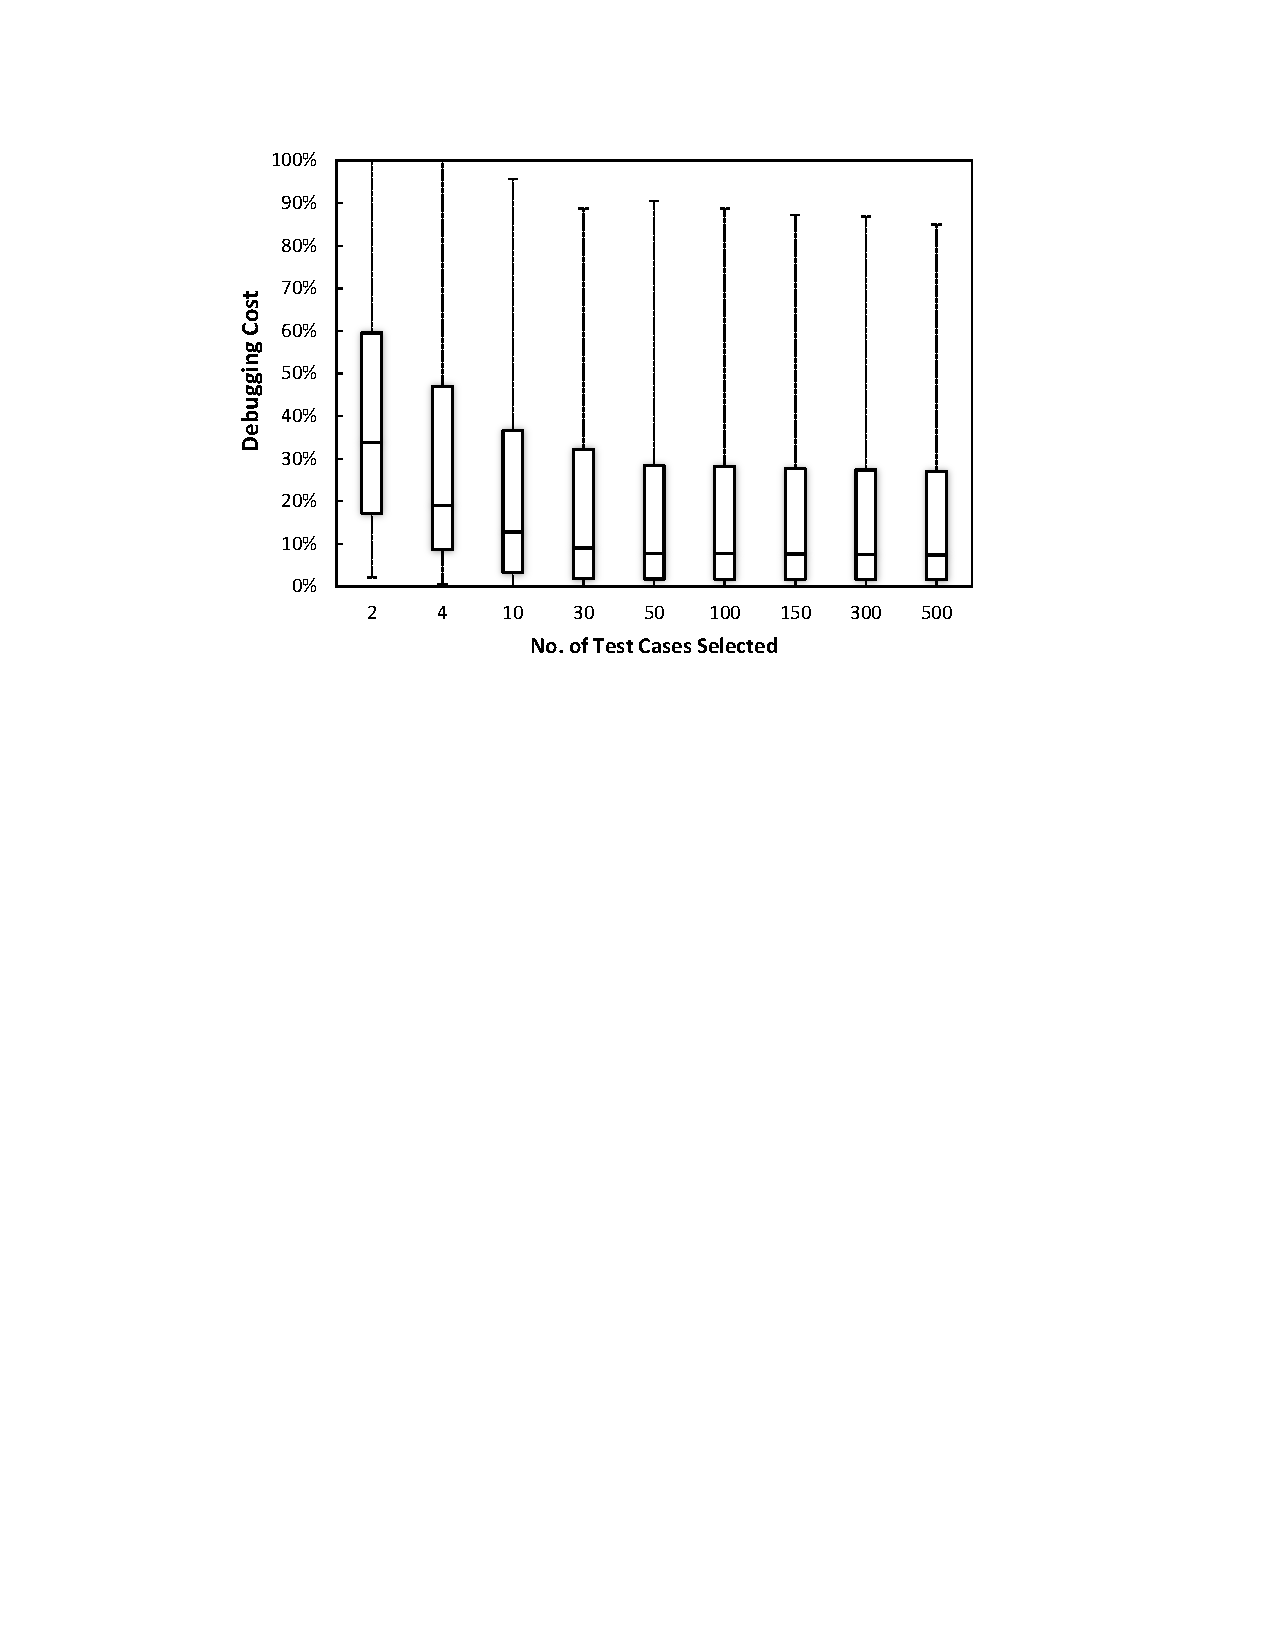
\includegraphics[width=12cm]{sdm_boxplot.pdf}
   % \vspace*{-12pt}
    \caption{Average Cost of {\sc Dms} when Selecting Different Numbers of Test Cases.}
    \label{Dms_boxplot}
\end{figure}

Following \cite{BaahPH10,BaahPH11} and the {\em cost}
metric (Equation~\ref{equation.avgcost}), we compare
the effectiveness of two prioritization methods $P_A$ and $P_B$ by using
one of the methods (for example, $P_B$) as reference measure.
When selecting the same number of traces $k$, the cost difference:
$cost(P_B) - cost(P_A)$ is considered as the improvement of $P_A$
over $P_B$. A positive value means that $P_A$ performs better than
$P_B$ (since lower cost is better) and a negative value means that the performance deteriorates if we use $P_A$ to replace $P_B$.
The difference corresponds
to the magnitude of improvement. For example, if the cost of
test cases from $P_A$ is 30\% and the cost of $P_B$ is 40\%,
then the improvement of $P_A$ over $P_B$ is 10\%, which means
that developers would examine 10\% fewer statements if $P_A$
is deployed.

\vspace{0.2cm}
\noindent{\bf Result Summary.} Table \ref{tab:compare_11}, \ref{tab:compare_21}, and \ref{tab:compare_31} compare
our method with the existing prioritizing techniques. The results show that
our method outperforms no worse than other methods for the majority of faulty program versions.

%\vspace{-0.1cm}
\begin{table}[tbp]
%	\vspace{-8pt}
    \centering
		\caption{Comparison of Prioritization methods.}
		\renewcommand{\arraystretch}{1.5}
		\small
        \begin{tabular}{|c|c|c|c|}
			\hline
			Test Prioritization Method  &  Positive  &  Negative  &   Neutral  \\
			\hline\hline
			\textsc{Dms} vs \textsc{Raptor} & {\bf 25.20\%} &    19.29\% &    55.51\% \\
			\hline
			\textsc{Dms} vs \textsc{Sequoia} & {\bf 33.46\%} &    19.69\% &    46.85\% \\
			\hline
			\textsc{Dms} vs \textsc{Stmt-Addtl} & {\bf 42.13\%} &    19.29\% &    38.58\% \\
			\hline
			\textsc{Dms} vs \textsc{Stmt-Total} & {\bf 62.99\%} &     7.87\% &    29.13\% \\
			\hline
			\textsc{Dms} vs \textsc{Fep-Addtl} & {\bf 40.16\%} &    20.08\% &    39.76\% \\
			\hline
			\textsc{Dms} vs \textsc{Art-Min} & {\bf 31.50\%} &    19.29\% &    49.21\% \\
			\hline
		\end{tabular}
    \label{tab:compare_11}
\end{table}

%\vspace{-0.1cm}
As illustrated in Table \ref{tab:compare_11}, \textsc{Dms} performs
better than \textsc{Raptor} on 25.20\% of the faulty versions, worse
on 19.29\% of the faulty versions, and shows no improvement
on 55.51\% of the faulty versions. The first row of
Table \ref{tab:compare_21} characterizes the degree of positive improvement of
\textsc{Dms} over \textsc{Raptor}. As the table indicates, half of the 25.20\%
faulty versions with positive improvement values have improvements
between 0.03\% and 3.93\%, and the other half
have improvements between 3.93\% and 77.42\%. The average
positive improvement of \textsc{Dms} over \textsc{Raptor} is 7.71\%.

%\vspace{-0.1cm}
\begin{table}[tbp]
    \centering
		\caption{Distribution of positive improvements.}
		\renewcommand{\arraystretch}{1.5}
		\small
        \begin{tabular}{|c|c|c|c|c|}
			\hline
			Test Pri. Tech.  &        Max &       Mean &     Median &        Min \\
			\hline\hline
			\textsc{Dms} vs \textsc{Raptor} & {\bf 77.42\%} &     7.71\% &     3.93\% &     0.03\% \\
			\hline
			\textsc{Dms} vs \textsc{Sequoia} & {\bf 66.67\%} &    14.38\% &     8.06\% &     0.23\% \\
			\hline
			\textsc{Dms} vs \textsc{Stmt-Addtl} & {\bf 72.87\%} &    14.68\% &     5.17\% &     0.03\% \\
			\hline
			\textsc{Dms} vs \textsc{Stmt-Total} & {\bf 94.97\%} &    27.68\% &    22.29\% &     0.03\% \\
			\hline
			\textsc{Dms} vs \textsc{Fep-Addtl} & {\bf 45.90\%} &    13.83\% &     6.35\% &     0.03\% \\
			\hline
			\textsc{Dms} vs \textsc{Art-Min} & {\bf 53.81\%} &     7.70\% &     3.23\% &     0.03\% \\
			\hline
		\end{tabular}
    \label{tab:compare_21}
\end{table}

Table \ref{tab:compare_31} characterizes the degree of negative deterioration of
\textsc{Dms} over other techniques. As the first row in the table indicates, for half of the 19.29\%
faulty versions, {\sc Dms} deteriorates 
% with positive improvement values have improvements
between 0.03\% and 0.60\% from \textsc{Raptor}, and for the other half,
%have improvements 
{\sc Dms} deteriorates between 0.60\% and 1.15\%. The average
percentage of negative deterioration of \textsc{Dms} over \textsc{Raptor} is 0.54\%.

\begin{table}[tbp]
    \centering
		\caption{Distribution of negative deterioration.}
		\renewcommand{\arraystretch}{1.5}
		\small
        \begin{tabular}{|c|c|c|c|c|}
			\hline
			Test Pri. Tech.  &        Max &       Mean &     Median &        Min \\
			\hline\hline
			\textsc{Dms} vs \textsc{Raptor} & {\bf 1.15\%} &     0.54\% &     0.60\% &     0.03\% \\
			\hline
			\textsc{Dms} vs \textsc{Sequoia} & {\bf 31.71\%} &    4.01\% &     1.33\% &     0.03\% \\
			\hline
			\textsc{Dms} vs \textsc{Stmt-Addtl} & {\bf 30.73\%} &    4.14\% &     1.52\% &     0.03\% \\
			\hline
			\textsc{Dms} vs \textsc{Stmt-Total} & {\bf 27.88\%} &    4.61\% &    2.64\% &     0.17\% \\
			\hline
			\textsc{Dms} vs \textsc{Fep-Addtl} & {\bf 24.70\%} &    5.06\% &     2.15\% &     0.03\% \\
			\hline
			\textsc{Dms} vs \textsc{Art-Min} & {\bf 22.41\%} &     4.11\% &     1.72\% &     0.03\% \\
			\hline
		\end{tabular}
    \label{tab:compare_31}
\end{table}


We conduct paired Wilcoxon signed-rank test to confirm the difference in performance between \textsc{Dms} and six existing prioritization techniques.
The statistical test result rejects the null hypothesis and suggests that the improvements of \textsc{Dms} over other existing techniques 
are statistically significant
%better than the existing best approach on \textsc{Unix} programs 
at 95\% confidence interval.

\vspace{0.2cm}
\noindent{\bf Detailed Comparison.} Table \ref{tab:label_effort} shows that \textsc{Raptor}, \textsc{Fep-Addtl} and \textsc{Art-Min} achieve 101\% of base line effectiveness with less than 500 test cases on subject programs.
Figure~\ref{fig:our_vs_fep}, \ref{fig:our_vs_artmin}, and~\ref{fig:our_vs_ag_unix}
show the comparison of fault localization costs between {\sc Dms} and the three different
prioritization techniques.
The horizontal axes represent the number of versions that
show differences in the Cost of
fault localization. The vertical axes represent the percentage
difference in Costs. If \textsc{Dms} is better than the reference
method, the area above zero-level line will be larger.

\vspace{0.2cm}
\noindent{\it D{\scriptsize MS} vs F{\scriptsize EP}-A{\scriptsize DDTL}.}
Previous studies~\citep{RUCH01,SEAGMGR01} show that \textsc{Fep-Addtl} is the most
promising prioritizing method for fault detection.
%However \textsc{Fep-Addtl} is not suitable for diagnostic prioritization,
%since it is initially proposed for regression testing, which assumes that
%tester have already get test oracles for each test case. But measuring
%{\em FEP} requires test oracles for all test cases which are absent in our problem.
%As a result, without test oracles {\em FEP} cannot evaluate the fault
%detection rate of each test case on program mutants.
%To circumvent this problem, Alberto \etal~\citep{Gonzalez-SanchezPAGG11} approximated {\em FEP}
Without test oracles, \textsc{Fep} can be estimated by $1 - ${\em False Negative Rate} (\textsc{Fnr})~\citep{Gonzalez-SanchezPAGG11}
\footnote{\textsc{Fnr} is the program passing rate when program element is the real fault and executed in test case. Usually when
\textsc{Fnr} is high, the fault is difficult to be detected by Spectrum-based
fault localization techniques.} which is also used in our study.
Figure \ref{fig:our_vs_fep} presents the comparison
between \textsc{Dms} and \textsc{Fep-Addtl} over all faulty versions that show performance differences.
\textsc{Fep-Addtl} is used as the reference prioritization technique.
The baseline represents the fault localization cost on program spectra prioritized
by \textsc{Fep-Addtl}. Each program version is a bar in this graph and we remove
versions from the graph that have no cost differences.
In the figure, the vertical axis represents the magnitude of
improvement of \textsc{Dms} over \textsc{Fep-Addtl}.
If the bar of a faulty version is above the
horizontal axis, that means on this version \textsc{Dms} performs
better than \textsc{Fep-Addtl} (positive improvement) and the bars
below the horizontal axis represent faulty versions for which
\textsc{Dms} performs worse than \textsc{Fep-Addtl}.

\begin{figure}[tbp]
    \centering
    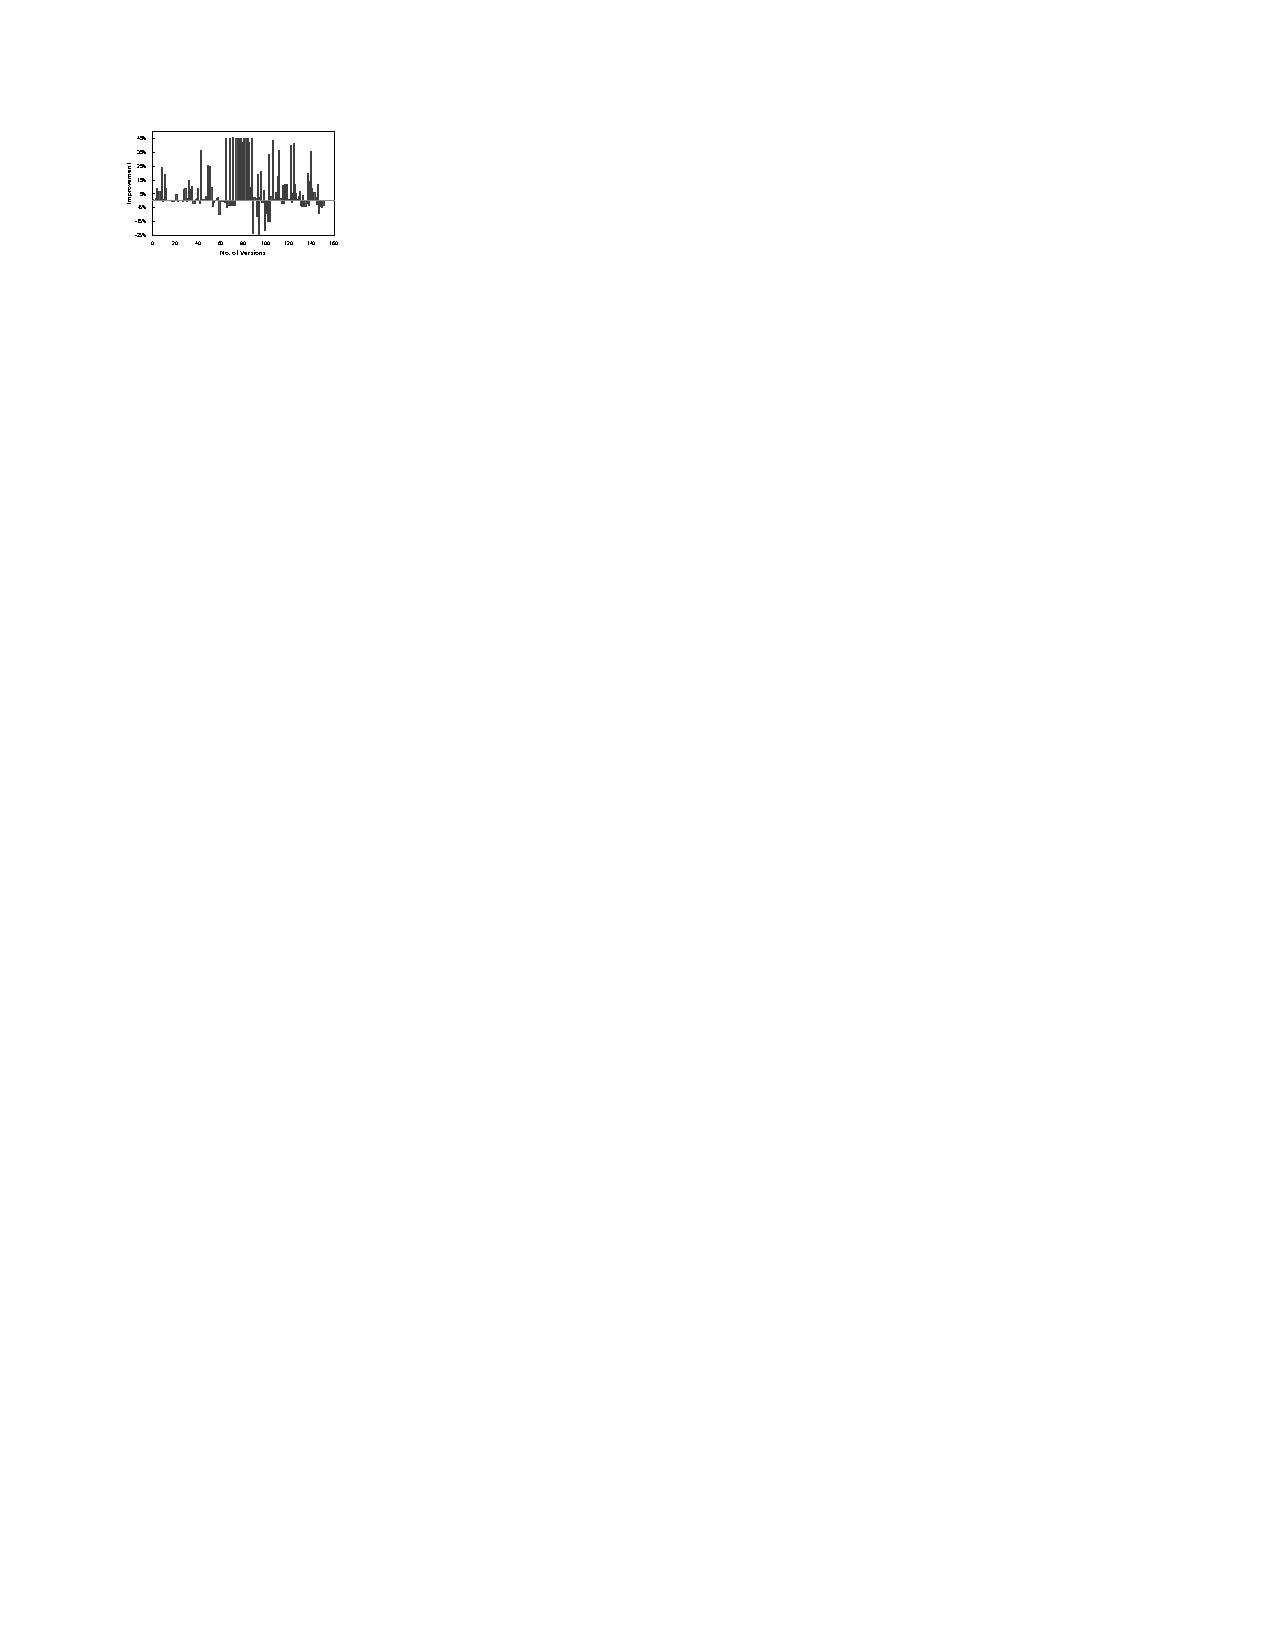
\includegraphics[width=12cm]{our_vs_fep.pdf}
%    \vspace{-0.3cm}
    \caption{Improvement of D{\scriptsize MS} over F{\scriptsize EP}-A{\scriptsize DDTL}.}
    \label{fig:our_vs_fep}
\end{figure}
%\vspace{0.2cm}

The comparison shows that \textsc{Dms} performs better than \textsc{Fep-Addtl} 
%for the majority of faulty versions.
%, our prioritization method performs
%better than \textsc{Fep-Addtl} 
on 102 versions, out of 153 versions that show differences in cost, but performs worse than
\textsc{Fep-Addtl} on 51 versions.
The positive improvement ranges from 0.03\% to 45.90\%, with an average of 6.35\%.


\begin{figure}[tbp]
    \centering
    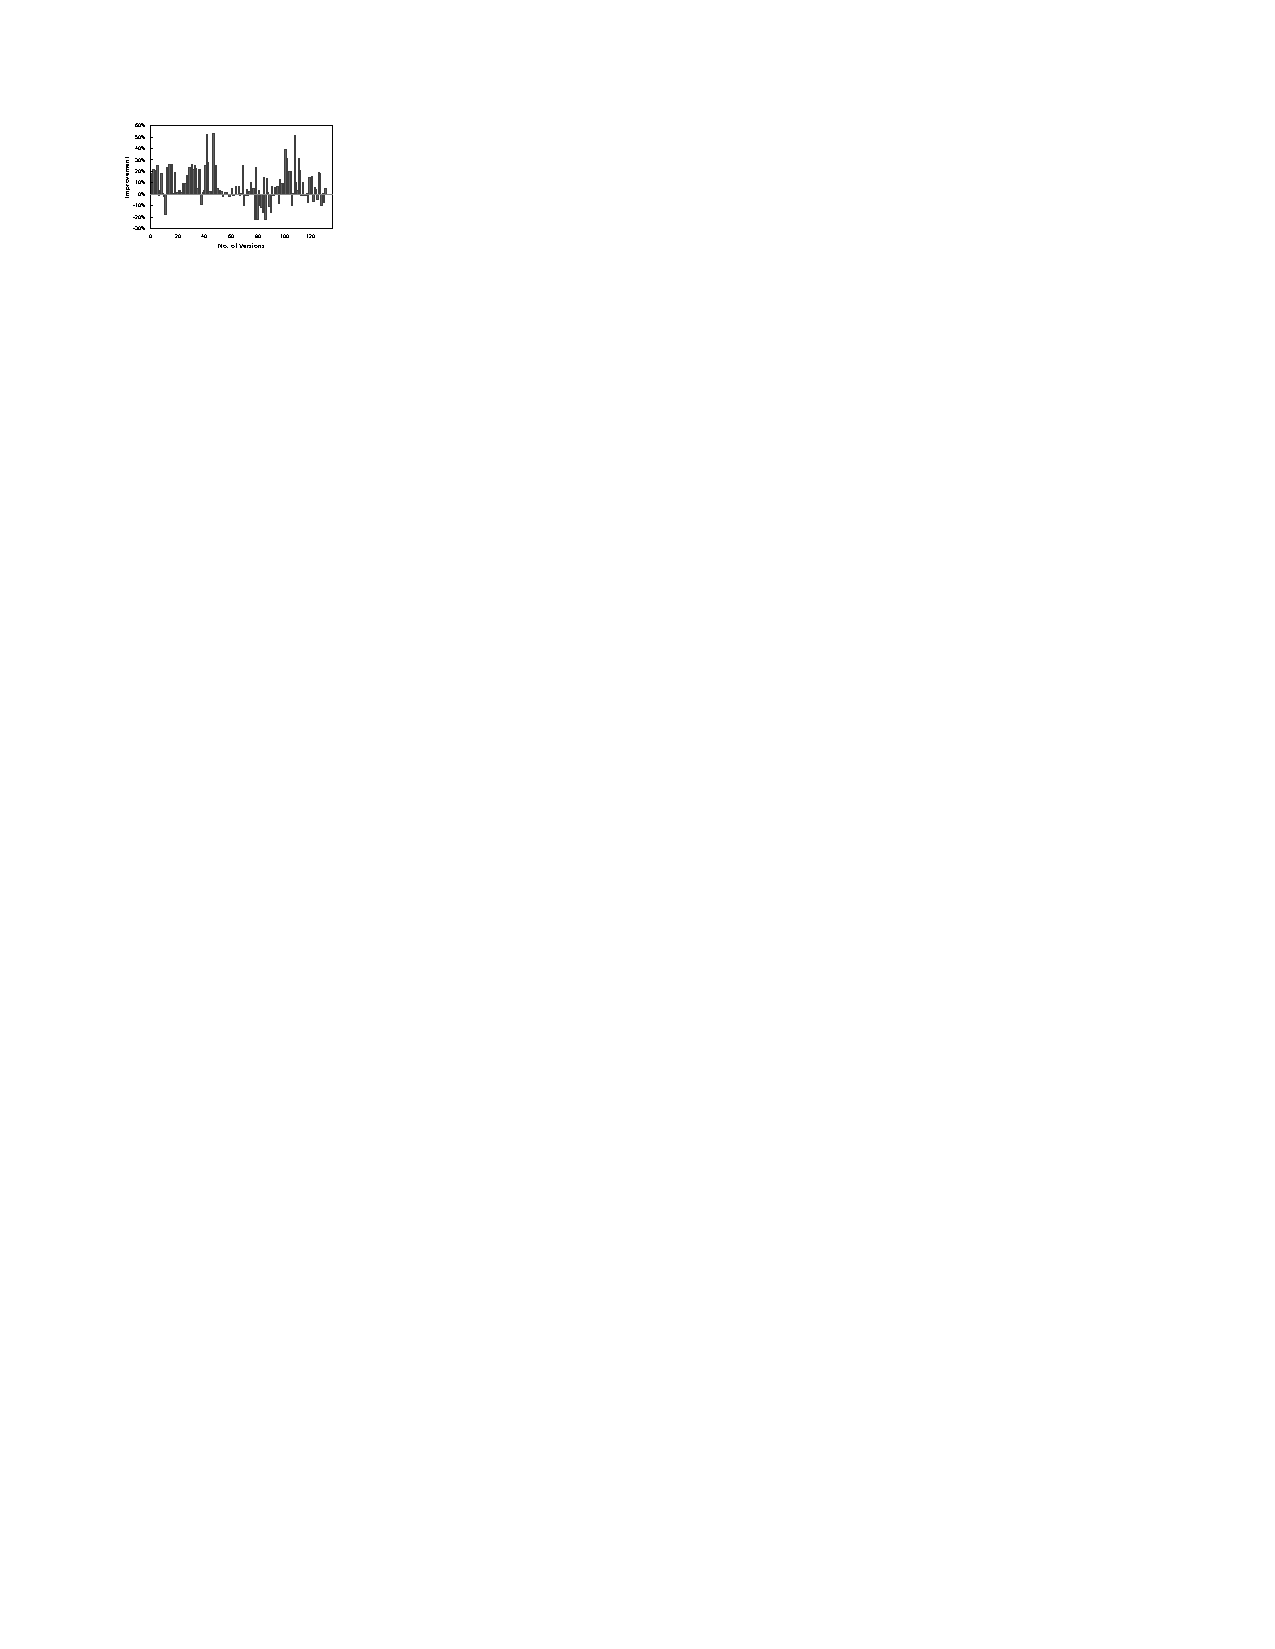
\includegraphics[width=12cm]{our_vs_artmin.pdf}
%    \vspace{-0.3cm}
    \caption{Improvement of D{\scriptsize MS} over A{\scriptsize rt}-M{\scriptsize IN}.}
    \label{fig:our_vs_artmin}
\end{figure}

\vspace{0.2cm}
\noindent{\it D{\scriptsize MS} vs A{\scriptsize rt}-M{\scriptsize IN}.} In this study we compare the effectiveness of \textsc{Dms} to {\em Adaptive Random Test Prioritization}(\textsc{Art})~\citep{JiangZCT09}.
There are various strategies for \textsc{Art}, in this experiment we only compare with the best one: \textsc{Art-Min}~\citep{JiangZCT09, Gonzalez-SanchezPAGG11, Alberto2011}.
Figure \ref{fig:our_vs_artmin} shows the results of the study in which \textsc{Art-Min} is used
as the baseline method. The comparison shows that \textsc{Dms} is better than \textsc{Art-Min}.
Out of 129 versions that show differences in cost, our prioritization method performs
better than \textsc{Art-Min} on 80 versions but performs worse than the
\textsc{Art-Min} on 49 versions.
%The positive improvement ranges from 0.03\% to 53.81\%, with an average of 7.70\%.

\vspace{0.2cm}
\noindent{\it D{\scriptsize MS} vs R{\scriptsize APTOR}.}
Figure \ref{fig:our_vs_ag_unix} shows the comparison between \textsc{Dms} and \textsc{Raptor} on \textsc{Unix} programs.
Here we use \textsc{Raptor} as the reference metric. The comparison shows that \textsc{Dms} 
%is better than \textsc{Raptor}.
%On \textsc{Unix} programs, 
outperforms \textsc{Raptor} on 20 versions by at least 1\% cost,
and on only 5 versions, it is worse than {\sc Raptor} by over 1\% cost.

\begin{figure}[tbp]
    \centering
    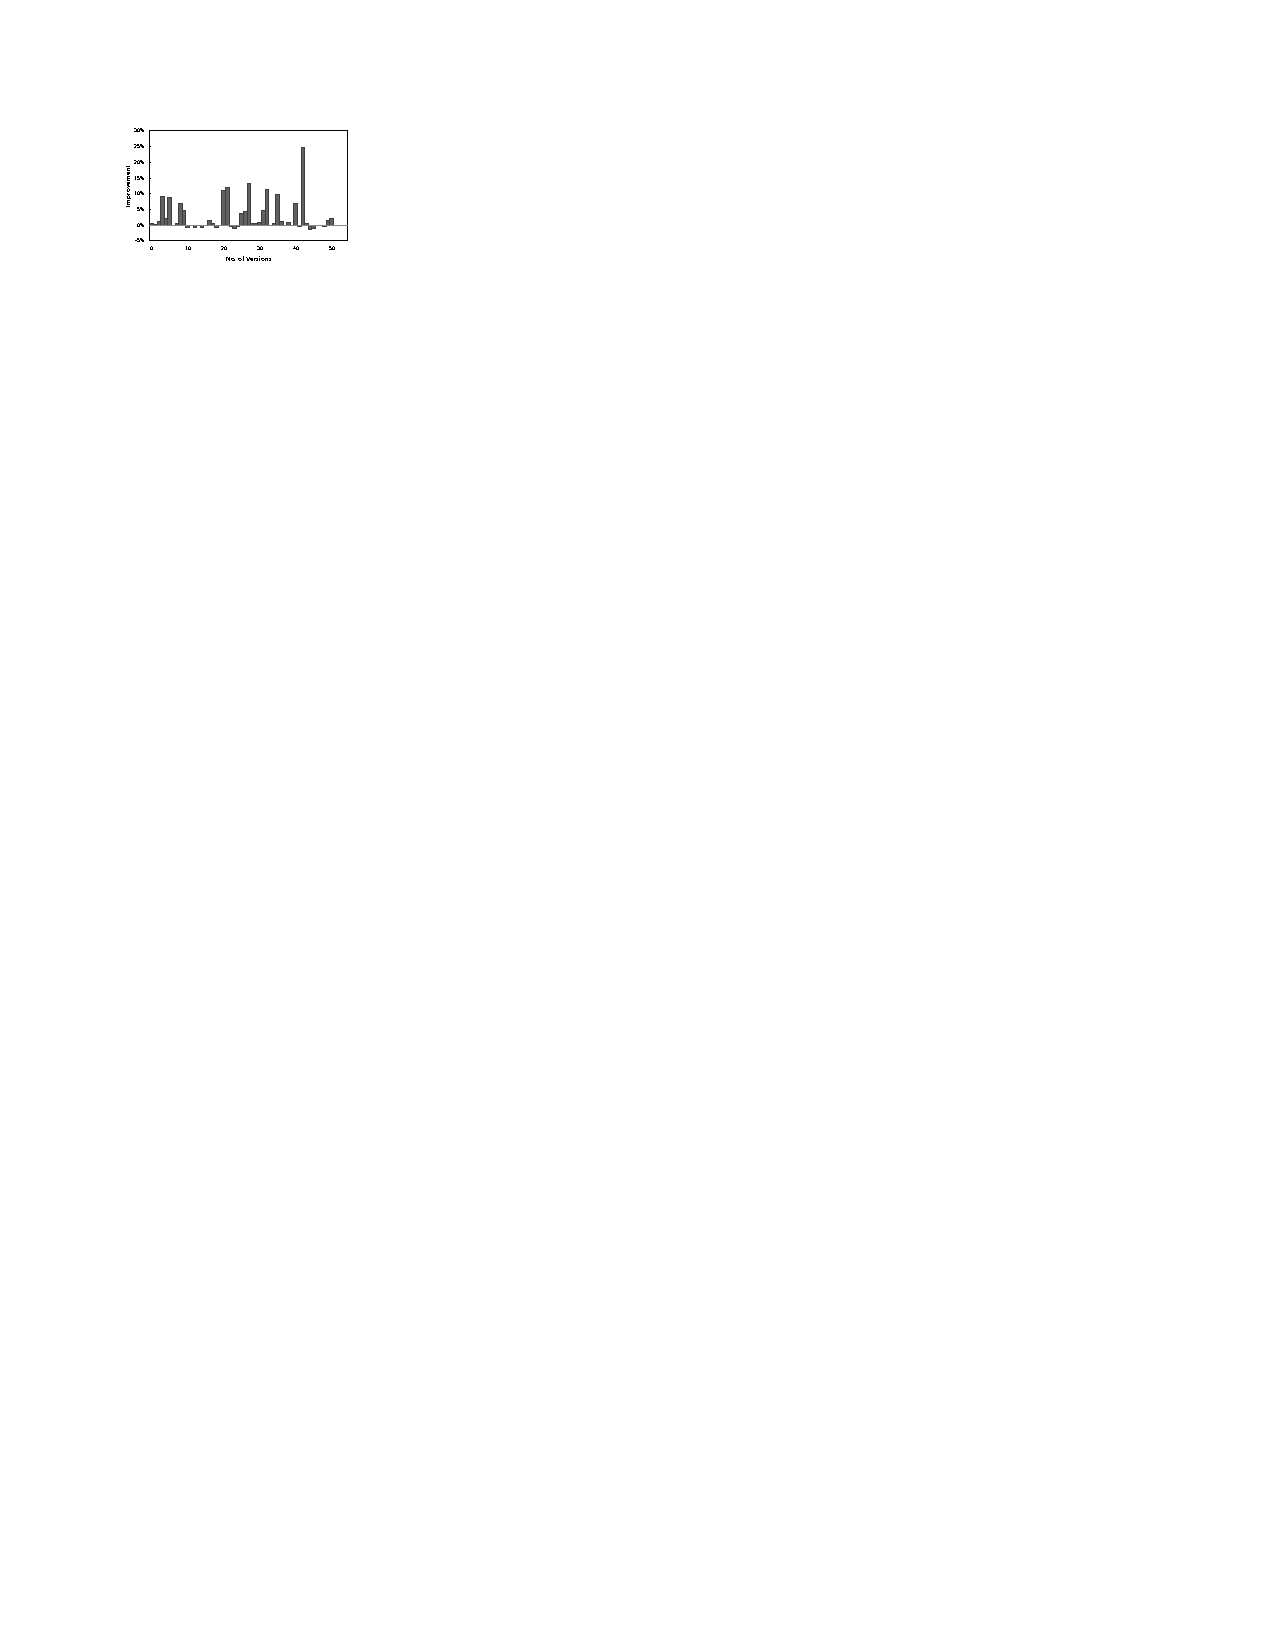
\includegraphics[width=12cm]{our_vs_ag_unix.pdf}
%    \vspace{-0.3cm}
    \caption{Improvement of D{\scriptsize MS} over R{\scriptsize APTOR} on U{\scriptsize NIX} programs.}
    \label{fig:our_vs_ag_unix}
\end{figure}

There is also improvement on Siemens programs: 32.2\% versions show differences and the average debugging cost improvement is 1.3\%, which is not so significant as compared with \textsc{Unix} programs.
This is probably due to the small software size. On Siemens programs, {\sc Raptor}
can reach 101\% of base line effectiveness by only selecting 20 test cases on average (see Table \ref{tab:label_effort}).
By selecting such few test cases, \textsc{Raptor} already obtains the maximal ambiguity group reduction due to very limited different
coverage profiles. For example, all test cases of \texttt{tcas} only have less than 15 ambiguity groups in all faulty versions. In this case,
the speedup by our method is trivial. In real scenario, programs to be diagnosed would be more similar to \textsc{Unix} programs.


\subsection{RQ2: multi-fault Programs}\label{sec.rq2}
Section~\ref{sec.exp.setup2} gives details about our experimental setup for multi-fault programs. Section~\ref{sec.exp.subject2} introduces the subject programs used in our study. Sections~\ref{sec.exp.resultsA2}~\&~\ref{sec.exp.resultsB2} show the results.

\subsubsection{Experimental Setups and Measures}\label{sec.exp.setup2}

The overall experimental setups and measures used for comparison for the multi-fault setting is similar to the single-fault setting. 

There is only a minor difference in the definition of the diagnostic cost as now there are multiple faults. The diagnostic cost is defined as follows:

\begin{equation}\label{equation.avgcost.multifault}
	cost = \dfrac{\left|  \left\{ j \left| \right.
           f_{T_{\mathcal{S}}}(d_j) \geq \min_{\substack{d_* \in D*}} f_{T_{\mathcal{S}}}(d_*) \right\} \right|}
           {\left|  \mathcal{D} \right|}
\end{equation}
where $\mathcal{D}$ consists of all program elements appearing in the program and $D_*$ is a set of faults in a program.
We calculate the average cost as the percentage of elements that developers have
to examine until locating all root causes ($D_*$). Since multiple
program elements can be assigned with the same suspiciousness score, the numerator
is considered as the number of program elements $d_j$ that have bigger or the
same suspiciousness score to a root cause $d_*$ in $D_*$ with the
lowest
%ambiguousness
suspiciousness
score. In this setting, we consider the worst-case scenario where developers need
to find all root causes by inspecting all elements that have a score no lower than the score of {\em any} root cause.

%In our experiment, every test case prioritization technique starts from an arbitrary labeled failed trace because developers start debugging only when test cases fail.

%We compare the effectiveness of different prioritization methods based on the diagnostic cost when the same number of test cases are selected.

%The diagnostic cost is defined as follows:
%\begin{equation}\label{equation.avgcost}
%	cost = \dfrac{\left|  \left\{ j \left| \right. f_{T_{\mathcal{S}}}(d_j) \geq f_{T_{\mathcal{S}}}(d_*) \right\}  \right|}{\left|  \mathcal{D} \right|}
%\end{equation}
%where $\mathcal{D}$ consists of all program elements appearing in the program.
%We calculate the average cost as the percentage of elements that developers have
%to examine until locating the root cause($d_*$) of failure. Since multiple
%program elements can be assigned with the same suspicious score, the numerator
%is considered as the number of program elements $d_j$ that have bigger or the
%same suspicious score to $d_*$.
%
%In this paper, we use \textsc{Raptor} as the bootstrapping technique ($\mathcal{P}$ in Figure \ref{algo:DMS}). During the bootstrapping process, $w$ is set to 10 to facilitate trend analysis.
%
%Following~\cite{JiangCT11}, for each faulty version, we repeat each prioritization technique 20 times to obtain its average cost. For each time, a randomly chosen failed trace is used as the starting point to alleviate the sensitivity of the technique to the choice of starting traces. On the other hand, to fairly compare our approach with other prioritization methods, the {\em same randomly} chosen failed traces are used as the starting traces for all methods.

\subsubsection{Subject Programs}\label{sec.exp.subject2}

Each multi-fault program version used in our study contains more than one fault where each fault involves only one line (or one simple statement if the statement is broken into more than one line) in the program and different faults affect different lines. This consideration is aligned with previous studies \citep[e.g.][]{zhang2013bridging,Abreu:2009.jss}. We use a dataset containing 173 multi-fault versions of 8 C programs as shown in Table~\ref{tab:multibug}. Different versions may contain the same fault, and there are 157 distinct faults in total. The dataset was previously used by \cite{lucia2013} to evaluate 40 different association measures.

%As print_token and schedule2 datasets only have four and seven bugs that involve one line, we randomly insert two bugs for every version, whereas for other datasets, we randomly insert five bugs for every multiple-bug version. Also, we ensure that each bug has been inserted at least in one of the versions. We generate multiple-bug versions for each dataset as many as the number of single-bug versions in the dataset. For example, there are 38 single-bug versions for Space, so we randomly generate 38 multiple-bug versions for Space, each of which contains five bugs. For each print_tokens and schedule2 dataset, we generate 10 multiple-bug versions. Thus, we have 20 multiple-bug versions that contain two bugs (minimum number of multiple bugs) and 153 versions that contain five bugs.

\begin{table}[!htbp]
	%\vspace{-8pt}
	\centering
	\caption{multi-fault Subject Programs}\label{tab:multibug}
	\renewcommand{\arraystretch}{1.5}
	%\small
    \begin{tabular}{|l|c|c|c|} \hline
        Program & \# Bugs Per Version &\# Tests& \# Versions\\ \hline\hline
		tcas & 5 &1,608& 41\\ \hline
        schedule2 & 2& 2,710 & 10\\ \hline
        schedule & 5&2,650 & 9\\ \hline
        replace & 5&5,542 & 32\\ \hline
		tot\_info & 5 &1,052 & 23\\ \hline
        print\_tokens2 & 5 &4,115& 10\\ \hline
        print\_tokens & 2&4,130 & 10\\ \hline
        space & 5&1,343 & 38\\ \hline
	\end{tabular}
\end{table}


%We use five real {\em C} programs and seven Siemens test programs from the {\em Software-artifact Infrastructure Repository}~(SIR)~\cite{doESE05}. We refer to the five real programs (\texttt{sed}, \texttt{flex}, \texttt{grep}, \texttt{gzip}, and \texttt{space}) as \textsc{Unix} programs. Table \ref{dataset} shows the descriptive statistics of each subject, including the number of faults, available test cases and code size. Following \cite{JHS02,Abreu:2009.jss}, we exclude faults not directly observable by the profiling tool\footnote{http://gcc.gnu.org/onlinedocs/gcc/Gcov.html} (e.g., some faults lead to a crash before \texttt{gcov} dumps profiling information and some faults do not cause any test case to fail), and in total we study 254 faults.


\subsubsection{Experimental Results: Reducing Number of Test Cases}\label{sec.exp.resultsA2}
%In this subsection, we conduct several controlled experiments to show the effectiveness of \textsc{Dms}.

%\vspace{-4pt}
%\subsubsubsection{Effectiveness on Reducing The Number of Test Cases Needed for a Target Cost}

We investigate the effectiveness of \textsc{DMS} in reducing the number of test cases needed for a targeted diagnostic cost for our multi-fault subject programs. Table \ref{tab:label_effort2} shows how many labels are needed on average to achieve 101\% of base line effectiveness (cf.\ Section \ref{sec.exp.setup}) for each approach. For example, \textsc{Raptor} requires 98 labels on average for each faulty version from all of the eight program datasets while \textsc{Dms} needs 79. In total, \textsc{Dms} requires the least amount of labeling effort; in comparison with the existing best approach (\textsc{FepAddtl}), \textsc{Dms} achieves 5.95\% labeling reduction on all of the datasets.

\begin{table}[!htbp]
%	\vspace{-8pt}
	\centering
	\caption{Labeling Effort on Subject Programs}
{
	\scriptsize
		\renewcommand{\arraystretch}{1.5}
		\hspace{-10pt}
        \begin{tabular}{|m{29pt}|m{13pt}|c|c|m{21pt}|m{21pt}|m{21pt}|m{17pt}|}
		   \hline
		     Subject &             &                &           & \textsc{Stmt-} & \textsc{Stmt-} & \textsc{Fep-}  & \textsc{Art-} \\
		   Programs & \textsc{Dms} & \textsc{Raptor}  & \textsc{Sequoia} & \textsc{Addtl} & \textsc{Total} & \textsc{Addtl} & \textsc{Min} \\
		   \hline\hline
		   All &   {\bf 79} &         98 &      111 &       102 &     240 &         84 &      164 \\
		   \hline
		 %  space &   {\bf 39} &         25&    72 &       48 &       305 &         71 &         73 \\
%		   \hline
		\end{tabular}
}
	\label{tab:label_effort2}
\end{table}


%\vspace{-6pt}
\subsubsection{Experimental Results: Reducing Cost}\label{sec.exp.resultsB2}
%\subsubsubsection{Effectiveness on Reducing Cost for a Given Number of Labeled Test Cases}

This subsection investigates the effectiveness of \textsc{Dms} in reducing cost given a targeted number of labeled test cases. Similar to the single-fault setting, we select 30 test cases and utilize the same method to compare between techniques. We also find that in our evaluation the average debugging cost of using \textsc{Dms} will not reduce significantly even if more labeled test cases than 50 are added further (see Figure \ref{fig:costmulti}).


\begin{figure}[tbp]
    \centering
    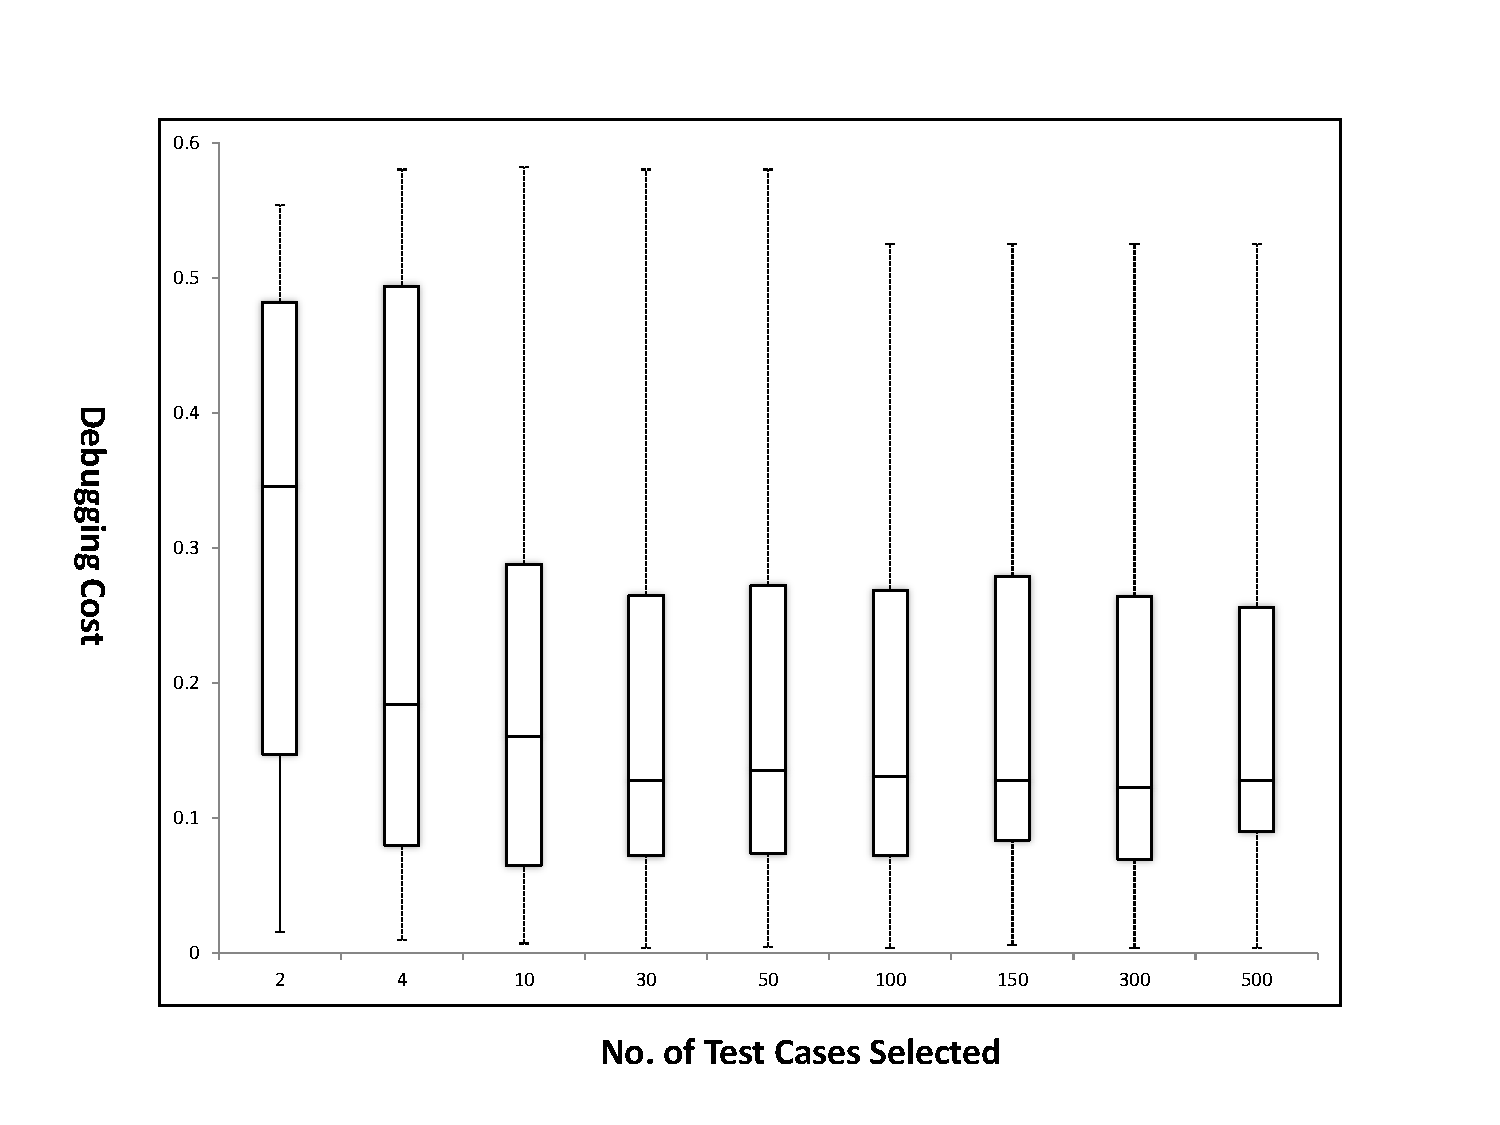
\includegraphics[width=12cm]{mut-sdm.pdf}
    %\vspace{-0.3cm}
    \caption{Average Cost of DMS when Selecting Different Numbers of Test Cases.}\label{fig:costmulti}

\end{figure}

\vspace{0.2cm}
\noindent{\bf Summary.} Table \ref{tab:compare_1}, \ref{tab:compare_2}, and~\ref{tab:compare_2_neg} summarize the comparison between our method and the existing prioritizing techniques.
%, the results show that our method outperforms all of them.
%\vspace{-0.1cm}
Table \ref{tab:compare_1} illustrates the distributions of {\sc Dms}'s performance against other techniques. For example, the first row shows that \textsc{Dms} performs better than \textsc{Raptor} on 34.68\% of the faulty versions, worse on 31.79\% of the faulty versions, and shows no improvement on 33.53\% of the faulty versions. The first row of Table~\ref{tab:compare_2} characterizes the degree of positive improvement of \textsc{Dms} over \textsc{Raptor}. As the table indicates, half of the 34.68\% faulty versions with positive improvement values have improvements between 0.03\% and 1.05\%, and the other half have improvements between 1.05\% and 46.75\%. The average positive improvement of \textsc{Dms} over \textsc{Raptor} is 5.95\%.
Table \ref{tab:compare_2_neg} illustrates the degree of negative deterioration of {\sc Dms} over other techniques. The first row shows that, half of the 31.79\% faulty versions for which {\sc Dms} performs worse than {\sc Raptor} have deterioration between 0.23\% and 2.94\%, and the other half have deterioration between 2.94\% and 53.30\%. The average deterioration of \textsc{Dms} from \textsc{Raptor} is 8.54\%.

\begin{table}[tbp]
%	\vspace{-8pt}
    \centering
		\caption{Comparison of Prioritization methods.}
		\renewcommand{\arraystretch}{1.5}
		\small
        \begin{tabular}{|c|c|c|c|}
			\hline
			Test Prioritization Method  &  Positive  &  Negative  &   Neutral  \\
			\hline\hline
			\textsc{Dms} vs \textsc{Raptor} & {\bf 34.68\%} &    31.79\% &    33.53\% \\
			\hline
			\textsc{Dms} vs \textsc{Sequoia} & {\bf 46.24\%} &    39.31\% &    14.45\% \\
			\hline
			\textsc{Dms} vs \textsc{Stmt-Addtl} & {\bf 50.29\%} &    28.23\% &    21.39\% \\
			\hline
			\textsc{Dms} vs \textsc{Stmt-Total} & {\bf 71.10\%} &    24.86\% &    4.05\% \\
			\hline
			\textsc{Dms} vs \textsc{Fep-Addtl} & {\bf 51.45\%} &   29.48\% &    19.08\% \\
			\hline
			\textsc{Dms} vs \textsc{Art-Min} & {\bf 71.68\%} &    23.70\% &    4.62\% \\
			\hline
		\end{tabular}
    \label{tab:compare_1}
\end{table}


\begin{table}[tbp]
    \centering
		\caption{Distribution of positive improvements.}
		\renewcommand{\arraystretch}{1.5}
		\small
        \begin{tabular}{|c|c|c|c|c|}
			\hline
			Test Prioritization Method  &        Max &       Mean &     Median &        Min \\
			\hline\hline
			\textsc{Dms} vs \textsc{Raptor} & {  46.75\%} &     5.95\% &     1.05\% &     0.03\% \\
			\hline
			\textsc{Dms} vs \textsc{Sequoia} & {  51.75\%} &   18.31\% &     14.31\% &     0.56\% \\
			\hline
			\textsc{Dms} vs \textsc{Stmt-Addtl} & {   54.24\%} &    10.67\% &     4.50\% &     0.04\% \\
			\hline
			\textsc{Dms} vs \textsc{Stmt-Total} & {  56.31\%} &    19.25\% &    25.42\% &     0.19\% \\
			\hline
			\textsc{Dms} vs \textsc{Fep-Addtl} & {  99.05\%} &    17.94\% &     9.04\% &     0.02\% \\
			\hline
			\textsc{Dms} vs \textsc{Art-Min} & {  99.13\%} &     42.96\% &     36.83\% &     0.14\% \\
			\hline
		\end{tabular}
    \label{tab:compare_2}
\end{table}


\begin{table}[tbp]
    \centering
		\caption{Distribution of negative deterioration.}
		\renewcommand{\arraystretch}{1.5}
		\small
        \begin{tabular}{|c|c|c|c|c|}
			\hline
			Test Prioritization Method  &        Max &       Mean &     Median &        Min \\
			\hline\hline
			\textsc{Dms} vs \textsc{Raptor} & {  53.30\%} &     8.54\% &     2.94\% &     0.23\% \\
			\hline
			\textsc{Dms} vs \textsc{Sequoia} & {  52.00\%} &   8.49\% &     4.37\% &     0.19\% \\
			\hline
			\textsc{Dms} vs \textsc{Stmt-Addtl} & {  53.86\%} &    10.88\% &     4.87\% &     0.14\% \\
			\hline
			\textsc{Dms} vs \textsc{Stmt-Total} & { 51.38\%} &   10.56\% &   7.10\% &     0.13\% \\
			\hline
			\textsc{Dms} vs \textsc{Fep-Addtl} & {  47.13\%} &    10.72\% &     5.89\% &     0.04\% \\
			\hline
			\textsc{Dms} vs \textsc{Art-Min} & {  46.21\%} &     3.33\% &     2.01\% &     0.16\% \\
			\hline
		\end{tabular}
    \label{tab:compare_2_neg}
\end{table}

We conduct paired Wilcoxon signed-rank test to confirm the difference in performance between \textsc{Dms} and six existing prioritization techniques. The statistical test result rejects the null hypothesis and suggests that the performance differences between \textsc{Dms} and other techniques are statistically significant
%ly better than the existing best approach on the multi-fault subject programs 
at 95\% confidence interval.

\vspace{0.2cm}\noindent{\bf Detailed Comparison.}
Similar to the single-fault setting, 
%Table \ref{tab:label_effort} shows that \textsc{Raptor}, \textsc{Fep-Addtl} and \textsc{Art-Min} achieve 101\% base line effectiveness with less than 500 test cases on subject programs. We only 
we show the comparison between \textsc{Dms} and three methods, \textsc{Raptor}, \textsc{Fep-Addtl} and \textsc{Art-Min}, in terms of fault localization costs in Figure~\ref{fig:our_vs_fep.multifault}, \ref{fig:our_vs_artmin.multifault}, and~\ref{fig:our_vs_raptor.multifault}.
%show the comparison between different prioritization techniques based on fault localization cost.

\vspace{0.2cm}\noindent{\it D{\scriptsize MS} vs F{\scriptsize EP}-A{\scriptsize DDTL}.}
Figure \ref{fig:our_vs_fep.multifault} presents the comparison between \textsc{Dms} and \textsc{Fep-Addtl} over all faulty versions that show cost differences. The comparison shows that \textsc{Dms} is better than \textsc{Fep-Addtl} on 89 versions, out of 140 versions that show differences in cost, 
but performs worse than the \textsc{Fep-Addtl} on 51 versions. The positive improvement ranges from 0.02\% to 99.05\%, with an average of 17.94\%.

%Previous studies~\cite{RUCH01,SEAGMGR01} show that \textsc{Fep-Addtl} is the most promising prioritizing method for fault detection.
%However \textsc{Fep-Addtl} is not suitable for diagnostic prioritization,
%since it is initially proposed for regression testing, which assumes that
%tester have already get test oracles for each test case. But measuring
%{\em FEP} requires test oracles for all test cases which are absent in our problem.
%As a result, without test oracles {\em FEP} cannot evaluate the fault
%detection rate of each test case on program mutants.
%To circumvent this problem, Alberto \etal~\cite{Gonzalez-SanchezPAGG11} approximated {\em FEP}
%Without test oracles, \textsc{Fep} can be estimated by $1 - ${\em False Negative Rate} (\textsc{Fnr})~\cite{Gonzalez-SanchezPAGG11}
%\footnote{\textsc{Fnr} is the program passing rate when program element is the real fault and executed in test case. Usually when
%\textsc{Fnr} is high, the fault is difficult to be detected by Spectrum-based
%fault localization techniques.} which is also used in our study.

%\vspace{0.2cm}
\vspace{0.2cm}\noindent{\it D{\scriptsize MS} vs A{\scriptsize rt}-M{\scriptsize IN}.}
We compare the effectiveness of \textsc{Dms} to the best variant of {\em Adaptive Random Test Prioritization}(\textsc{Art}), namely \textsc{Art-Min}~\citep{JiangZCT09, Gonzalez-SanchezPAGG11, Alberto2011}. Figure \ref{fig:our_vs_artmin.multifault} shows the results of the study in which \textsc{Art-Min} is used as the baseline method. The comparison shows that \textsc{Dms} is better than \textsc{Art-Min} on 124 versions, out of 165 versions that show differences in cost, 
but performs worse than the \textsc{Art-Min} on 41 versions.

%The positive improvement ranges from 0.03\% to 53.81\%, with an average of 7.70\%.

\vspace{0.2cm}\noindent{\it D{\scriptsize MS} vs R{\scriptsize APTOR}.}
Figure \ref{fig:our_vs_raptor.multifault} shows the comparison between \textsc{Dms} and \textsc{Raptor}. The comparison shows that \textsc{Dms} is better than \textsc{Raptor} on 60 versions, out of 115 versions that show differences in cost, 
but performs worse than the \textsc{Raptor} on 55 versions.
The average deterioration (8.54\%) of {\sc Dms} (Table \ref{tab:compare_2_neg} is higher than its average improvement (5.95\%) in comparison with {\sc Raptor} (Table \ref{tab:compare_2}), even though {\sc Dms} reduces the total labelling effort from 98 test cases to 79 (Table \ref{tab:label_effort2}). We are yet unclear about the reason causing the trade-off in the multi-fault programs. It is very intriguing future work to find ways to balance between labelling effort and diagnostic cost better.

%\textsc{Dms} outperforms \textsc{Raptor} on 20 versions by at least 1\% cost, and only 5 versions worse than \textsc{Raptor} over 1\% cost.

\begin{figure}[tbp]
    \centering
    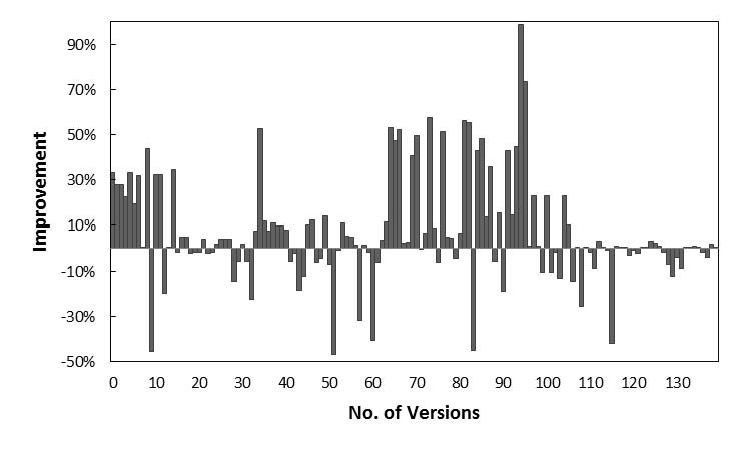
\includegraphics[width=12cm]{mut-dms-feq.pdf}
%    \vspace{-0.3cm}
\caption{Improvement of D{\scriptsize MS} over F{\scriptsize EP}-A{\scriptsize DDTL}.}
    \label{fig:our_vs_fep.multifault}
\end{figure}
%\vspace{0.2cm}



\begin{figure}[tbp]
    \centering
    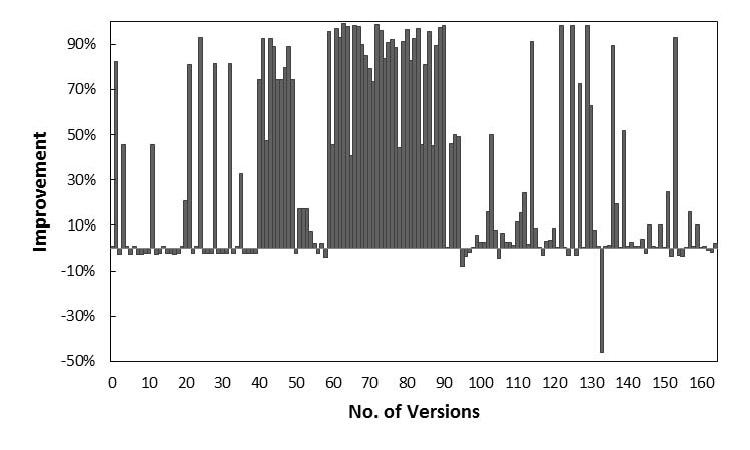
\includegraphics[width=12cm]{mut-dms-art.pdf}
%    \vspace{-0.3cm}
    \caption{Improvement of D{\scriptsize MS} over A{\scriptsize rt}-M{\scriptsize IN}.}
    \label{fig:our_vs_artmin.multifault}
\end{figure}

\begin{figure}[tbp]
    \centering
    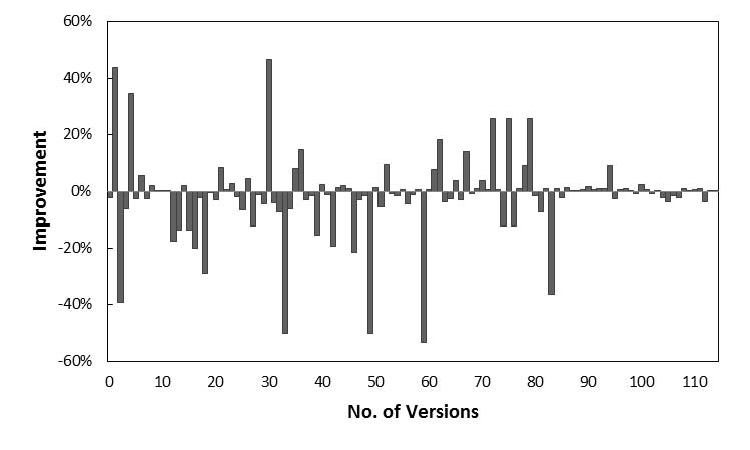
\includegraphics[width=12cm]{mut-dms-raptor.pdf}
%    \vspace{-0.3cm}
\caption{Improvement of D{\scriptsize MS} over R{\scriptsize APTOR}.}
    \label{fig:our_vs_raptor.multifault}
\end{figure}

%on U{\scriptsize NIX} programs

%There is also improvement on Siemens programs: 32.2\% versions show differences and the average debugging cost improvement is 1.3\%, which is not so significant as comparison on \textsc{Unix} programs.
%This is probably due to the small software size. On Siemens programs the existing best approach
%can reach 101\% of the base line effectiveness by only selecting less than 20 test cases on average (see Table \ref{tab:label_effort}).
%By selecting such few test cases, \textsc{Raptor} already obtains the maximal ambiguity group reduction due to very limited different
%coverage profiles. For example, all test cases of \texttt{tcas} only have less than 15 ambiguity groups in all faulty versions. In this case,
%the speedup by our method is trivial. In real scenario, programs to be diagnosed would be more similar to \textsc{Unix} programs.


\subsection{Discussion and Threats to Validity}\label{sec.exp.threats}
As we noticed, the improvement of \textsc{Dms} in single-fault and multi-fault programs are different. In the 12 single-fault programs,  \textsc{Dms} requires the minimal amount of labeling effort by achieving 67.7\% labeling reduction on Unix programs and 10\% reduction on Siemens programs in comparison with the existing best approach---Raptor. While in the 8 multi-fault programs, \textsc{Dms} achieves 5.95\% labeling reduction in comparison with the existing best approach---Fep-Addtl. The phenomenon happens since we consider the worst cases of \textsc{Dms} in multi-fault programs, i.e., we consider the root case $d_*$ with the lowest suspiciousness score. In some versions of the multi-fault programs, \textsc{Dms} needs more test cases to achieve the value of $c_x$ than that of Fep-Addtl. For example, in the version 2 of the program print\_token2, \textsc{Dms} need to label 500 test cases to achieve $c_x$, while Fep-Addtl only requires 59 test cases. Thus, the reduced number of test cases for \textsc{Dms} in multi-fault program is not as high as that in single-fault program.

However, the improvement of \textsc{Dms} in reducing cost is significant for both single-fault and multi-fault programs. The statistics of  paired Wilcoxon signed-rank test show that \textsc{Dms} is statistically significantly better than the existing best approach on the Unix programs of single-fault subject programs, and multi-fault subject programs at 95\% confidence interval. Moreover, although we notice that \textsc{Dms} reduce the number of test case of Fep-Addtl by 5.95\% in multi-fault programs, but there are 51.45\% fault versions that \textsc{Dms} show positive improvement over Fep-Addtl, and  29.48\% fault versions that \textsc{Dms} show negative improvement over Fep-Addtl, while the number for single-fault programs are 40.16\% and 20.08\%.


The threats to our studies include the issue of how
representative the subjects of our studies are. Since the Siemens programs
are small and larger programs may be subject to different testing and debugging traits.
To strengthen the external validity, we include \textsc{Unix} programs which are
real-life programs. These subjects have been adopted for evaluation in many
studies \citep[e.g.][]{JH05,Abreu:2009.jss,DBLP:conf/icse/SantelicesJYH09}.

Another possible threat is that although our method outperforms existing method
in 25.2\% to 62.99\% program versions and gets equivalent cost in around 30\% versions,
there are still a certain percent of versions that our method does not perform very well.
But as we can see in the studies, most of the negative improvements of those versions
are relatively small or even trivial comparing to the positive improvements. We also
conduct statistical test to further confirm the superiority of \textsc{Dms}.

%At last, the studies show that \textsc{Dms} outperforms other methods
%in reducing manual effort for debugging, but the ultimate
%merit should be evaluated by end-users. However, due to the
%expense as well as difficulty of user study, most existing works in
%test case prioritization and fault localization are temporarily evaluated
%by authors~\cite{RUCH01,SEAGMGR01,LHH07,Abreu:2009.jss}.

